%----------------------------------------------------------------------------------------
%    PACKAGES AND THEMES
%----------------------------------------------------------------------------------------
\documentclass[aspectratio=169,xcolor=dvipsnames]{beamer}
\makeatletter
\def\input@path{{../BeamerTemplate/theme/}}
\makeatother
\usetheme{CleanEasy}
\usepackage[utf8]{inputenc}
\usepackage{lmodern}
\usepackage[T1]{fontenc}
\usepackage{fix-cm}
\usepackage{amsmath}
\usepackage{mathtools}
\usepackage{listings}
\usepackage{xcolor}
\usepackage{hyperref}
\usepackage{graphicx}
\usepackage{booktabs}
\usepackage{tikz}
\usetikzlibrary{positioning, shapes, arrows, calc, decorations.pathreplacing, arrows.meta, backgrounds, patterns, overlay-beamer-styles}
\usepackage{etoolbox}

%----------------------------------------------------------------------------------------
%    LAYOUT CONFIGURATION
%----------------------------------------------------------------------------------------
\input{../BeamerTemplate/configs/configs}

%----------------------------------------------------------------------------------------
%    TITLE PAGE CONFIGURATION
%----------------------------------------------------------------------------------------
\title[Foundations]{Data Structures: Foundations}
\author{Minseok Jeon}
\institute{DGIST}
\date{\today}

% Simple title page without logos
\titlegraphic{}

%----------------------------------------------------------------------------------------

\begin{document}

\begin{frame}[plain]
  \titlepage
\end{frame}

\begin{frame}[plain]{Contents}
  \tableofcontents
\end{frame}

%----------------------------------------------------------------------------------------
%    INTRODUCTION
%----------------------------------------------------------------------------------------
\section{Introduction}

\begin{frame}{Why Foundations Matter}
  \begin{block}{Course Philosophy}
    Build a strong programming foundation \textbf{before} diving into complex data structures
  \end{block}

  \vspace{0.5cm}

  \begin{columns}
    \begin{column}{0.48\textwidth}
      \textbf{What You'll Master:}
      \begin{itemize}
        \item Programming language fundamentals
        \item Control flow and recursion
        \item Memory models (stack vs heap)
        \item Debugging and testing skills
        \item Problem-solving patterns
      \end{itemize}
    \end{column}
    \begin{column}{0.48\textwidth}
      \textbf{Why This Matters:}
      \begin{itemize}
        \item Data structures require solid coding skills
        \item Understanding memory is crucial
        \item Testing prevents subtle bugs
        \item Good habits accelerate learning
      \end{itemize}
    \end{column}
  \end{columns}

  \vspace{0.5cm}

  \begin{alertblock}{Key Principle}
    Implement every structure \textbf{from scratch} at least once to truly understand it
  \end{alertblock}
\end{frame}

%----------------------------------------------------------------------------------------
%    LANGUAGE CHOICE
%----------------------------------------------------------------------------------------
\section{Choosing a Programming Language}

\begin{frame}{Language Comparison}
  \begin{center}
    \begin{tabular}{l|p{3cm}|p{3.5cm}|p{3cm}}
      \toprule
      \textbf{Language} & \textbf{Strengths} & \textbf{Best For} & \textbf{Learning Curve} \\
      \midrule
      C/C++ & Maximum control, performance, STL & Competitive programming, systems & Steep (pointers, memory) \\
      \midrule
      Java & Strong libraries, OOP, widely used & Interviews, enterprise & Moderate \\
      \midrule
      Python & Readable, fast to write & Learning, prototyping & Easy \\
      \bottomrule
    \end{tabular}
  \end{center}

  \vspace{0.5cm}

  \begin{columns}
    \begin{column}{0.48\textwidth}
      \begin{block}{For Beginners}
        \textbf{Python} or \textbf{Java}
        \begin{itemize}
          \item Focus on concepts, not syntax
          \item Less memory management
          \item Faster iteration
        \end{itemize}
      \end{block}
    \end{column}
    \begin{column}{0.48\textwidth}
      \begin{block}{For Performance/CP}
        \textbf{C++}
        \begin{itemize}
          \item Learn STL containers
          \item Manual memory control
          \item Optimal execution speed
        \end{itemize}
      \end{block}
    \end{column}
  \end{columns}
\end{frame}

\begin{frame}[fragile]{Language-Specific Considerations}
  \begin{columns}
    \begin{column}{0.48\textwidth}
      \begin{exampleblock}{C++ Example}
        \begin{lstlisting}[language=C++,basicstyle=\tiny\ttfamily]
#include <vector>
#include <iostream>

int main() {
    std::vector<int> arr = {1, 2, 3};
    arr.push_back(4);  // Dynamic resize

    // Manual memory for complex types
    int* ptr = new int[100];
    delete[] ptr;  // Must free!

    return 0;
}
        \end{lstlisting}
        Manual memory, explicit types
      \end{exampleblock}
    \end{column}
    \begin{column}{0.48\textwidth}
      \begin{exampleblock}{Python Example}
        \begin{lstlisting}[language=Python,basicstyle=\tiny\ttfamily]
# Dynamic typing, GC
arr = [1, 2, 3]
arr.append(4)  # Auto-resize

# No manual memory management
# Objects cleaned up automatically

# But watch mutability!
list1 = [1, 2, 3]
list2 = list1  # Same reference
list2.append(4)
print(list1)  # [1, 2, 3, 4]
        \end{lstlisting}
        Automatic memory, dynamic types
      \end{exampleblock}
    \end{column}
  \end{columns}

  \vspace{0.3cm}

  \begin{alertblock}{Important}
    Data structures behave differently: manual memory in C/C++ vs garbage collection in Java/Python
  \end{alertblock}
\end{frame}

%----------------------------------------------------------------------------------------
%    CONTROL FLOW
%----------------------------------------------------------------------------------------
\section{Variables, Control Flow, and Loops}

\begin{frame}[fragile]{Core Concepts}
  \begin{columns}
    \begin{column}{0.48\textwidth}
      \begin{block}{Data Types \& Scope}
        \begin{itemize}
          \item Basic types: int, float, bool
          \item Type conversion and casting
          \item Variable scope and lifetime
        \end{itemize}
      \end{block}

      \vspace{0.2cm}

      \begin{exampleblock}{Control Flow}
        \begin{lstlisting}[language=Python,basicstyle=\tiny\ttfamily]
# If/else with early returns
def process(x):
    if x < 0:
        return "negative"
    elif x == 0:
        return "zero"
    else:
        return "positive"
        \end{lstlisting}
      \end{exampleblock}
    \end{column}
    \begin{column}{0.48\textwidth}
      \begin{block}{Loop Patterns}
        \begin{itemize}
          \item Index-based vs iterator-based
          \item Nested loops: O(n²), O(n³)
          \item Break/continue usage
          \item Loop invariants
        \end{itemize}
      \end{block}

      \vspace{0.2cm}

      \begin{exampleblock}{Common Pitfall}
        \begin{lstlisting}[language=Python,basicstyle=\tiny\ttfamily]
# Off-by-one error!
for i in range(len(arr) - 1):  # Missing last!
    print(arr[i])

# Correct:
for i in range(len(arr)):
    print(arr[i])
        \end{lstlisting}
      \end{exampleblock}
    \end{column}
  \end{columns}

  \vspace{0.3cm}

  \begin{alertblock}{Practice Problems}
    Sum array, find min/max, frequency count, reverse array, rotate array
  \end{alertblock}
\end{frame}

\begin{frame}[fragile]{Nested Loops and Complexity}
  \begin{exampleblock}{Time Complexity Examples}
    \begin{lstlisting}[language=Python,basicstyle=\small\ttfamily]
# O(n) - Single loop
for i in range(n):
    print(i)

# O(n^2) - Nested loop
for i in range(n):
    for j in range(n):
        print(i, j)

# O(n^3) - Triple nested
for i in range(n):
    for j in range(n):
        for k in range(n):
            print(i, j, k)
    \end{lstlisting}
  \end{exampleblock}

  \begin{alertblock}{Key Insight}
    Nested loops multiply complexity. Be aware of your algorithm's growth rate!
  \end{alertblock}
\end{frame}

%----------------------------------------------------------------------------------------
%    FUNCTIONS AND RECURSION
%----------------------------------------------------------------------------------------
\section{Functions and Recursion}

\begin{frame}[fragile]{Function Fundamentals}
  \begin{columns}
    \begin{column}{0.48\textwidth}
      \begin{block}{Key Concepts}
        \begin{itemize}
          \item Pass by value vs reference
          \item Return values and side effects
          \item Function purity
          \item Single responsibility principle
        \end{itemize}
      \end{block}

      \vspace{0.2cm}

      \begin{exampleblock}{Pure Function}
        \begin{lstlisting}[language=Python,basicstyle=\tiny\ttfamily]
# Pure: no side effects
def add(a, b):
    return a + b

# Impure: modifies state
def append_item(lst, item):
    lst.append(item)  # Side effect!
        \end{lstlisting}
      \end{exampleblock}
    \end{column}
    \begin{column}{0.48\textwidth}
      \begin{block}{Best Practices}
        \begin{itemize}
          \item Small, focused functions
          \item Clear, descriptive names
          \item Document preconditions
          \item Handle edge cases
        \end{itemize}
      \end{block}

      \vspace{0.2cm}

      \begin{exampleblock}{C++ Reference}
        \begin{lstlisting}[language=C++,basicstyle=\tiny\ttfamily]
// Pass by value (copy)
void func1(vector<int> v) {
    v.push_back(1);  // Original unchanged
}

// Pass by reference (no copy)
void func2(vector<int>& v) {
    v.push_back(1);  // Original modified
}
        \end{lstlisting}
      \end{exampleblock}
    \end{column}
  \end{columns}
\end{frame}

\begin{frame}[fragile]{Recursion Basics}
  \begin{block}{Essential Components}
    \begin{itemize}
      \item \textbf{Base case}: Stopping condition (prevents infinite recursion)
      \item \textbf{Recursive case}: Progress toward base case
      \item \textbf{Stack frames}: Each call adds to call stack
    \end{itemize}
  \end{block}

  \vspace{0.3cm}

  \begin{columns}
    \begin{column}{0.48\textwidth}
      \begin{exampleblock}{Factorial}
        \begin{lstlisting}[language=Python,basicstyle=\tiny\ttfamily]
def factorial(n):
    # Base case
    if n <= 1:
        return 1
    # Recursive case
    return n * factorial(n - 1)

# Call stack for factorial(3):
# factorial(3) -> 3 * factorial(2)
# factorial(2) -> 2 * factorial(1)
# factorial(1) -> 1 (base case)
# Unwind: 2 * 1 = 2, then 3 * 2 = 6
        \end{lstlisting}
      \end{exampleblock}
    \end{column}
    \begin{column}{0.48\textwidth}
      \begin{exampleblock}{Binary Search}
        \begin{lstlisting}[language=Python,basicstyle=\tiny\ttfamily]
def binary_search(arr, target, left, right):
    # Base case: not found
    if left > right:
        return -1

    mid = left + (right - left) // 2

    # Base case: found
    if arr[mid] == target:
        return mid

    # Recursive cases
    if arr[mid] > target:
        return binary_search(arr, target,
                           left, mid - 1)
    else:
        return binary_search(arr, target,
                           mid + 1, right)
        \end{lstlisting}
      \end{exampleblock}
    \end{column}
  \end{columns}
\end{frame}

\begin{frame}{Recursion Patterns and Pitfalls}
  \begin{columns}
    \begin{column}{0.48\textwidth}
      \begin{block}{Common Patterns}
        \begin{itemize}
          \item \textbf{Divide and Conquer}: \\
                Merge sort, quick sort
          \item \textbf{Tree Traversals}: \\
                In-order, pre-order, post-order
          \item \textbf{Backtracking}: \\
                Permutations, N-Queens
          \item \textbf{Dynamic Programming}: \\
                Fibonacci with memoization
        \end{itemize}
      \end{block}
    \end{column}
    \begin{column}{0.48\textwidth}
      \begin{alertblock}{Common Pitfalls}
        \begin{itemize}
          \item Missing base case \\
                $\rightarrow$ Infinite recursion
          \item Incorrect base case \\
                $\rightarrow$ Wrong results
          \item Deep recursion \\
                $\rightarrow$ Stack overflow
          \item No progress to base \\
                $\rightarrow$ Infinite loop
        \end{itemize}
      \end{alertblock}

      \vspace{0.2cm}

      \begin{block}{Solution for Deep Recursion}
        Convert to iterative with explicit stack
      \end{block}
    \end{column}
  \end{columns}

  \vspace{0.3cm}

  \begin{exampleblock}{Practice}
    Implement: factorial, Fibonacci (memoized), binary search (recursive/iterative), tree traversals
  \end{exampleblock}
\end{frame}

%----------------------------------------------------------------------------------------
%    ARRAYS AND STRINGS
%----------------------------------------------------------------------------------------
\section{Arrays and Strings Fundamentals}

\begin{frame}{Arrays: Core Properties}
  \begin{columns}
    \begin{column}{0.48\textwidth}
      \begin{block}{Key Characteristics}
        \begin{itemize}
          \item Contiguous memory
          \item O(1) indexing
          \item Fixed size vs resizable
          \item Cache-friendly
        \end{itemize}
      \end{block}

      \vspace{0.2cm}

      \begin{block}{Common Operations}
        \begin{tabular}{l|c}
          \textbf{Operation} & \textbf{Time} \\
          \hline
          Access & O(1) \\
          Search & O(n) \\
          Insert (end) & O(1) amortized \\
          Insert (middle) & O(n) \\
          Delete (middle) & O(n) \\
        \end{tabular}
      \end{block}
    \end{column}
    \begin{column}{0.48\textwidth}
      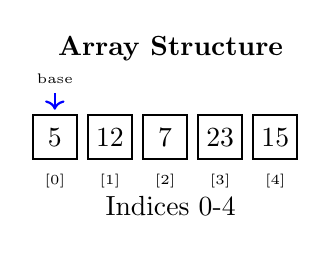
\begin{tikzpicture}[scale=0.7]
        % Array visualization
        \node at (2.5,3) {\textbf{Array Structure}};

        \foreach \i/\val in {0/5, 1/12, 2/7, 3/23, 4/15} {
          \draw[thick] (\i*1,1) rectangle (\i*1+0.8,1.8);
          \node at (\i*1+0.4,1.4) {\val};
          \node[below] at (\i*1+0.4,0.9) {\tiny[\i]};
        }

        \node[below] at (2.5,0.5) {Indices 0-4};

        \draw[->, thick, blue] (0.4,2.2) -- (0.4,1.9);
        \node[above] at (0.4,2.2) {\tiny base};
      \end{tikzpicture}

      \vspace{0.3cm}

      \begin{alertblock}{Memory Address}
        \texttt{addr[i] = base + i × size}
      \end{alertblock}
    \end{column}
  \end{columns}
\end{frame}

\begin{frame}[fragile]{Strings: Special Arrays}
  \begin{columns}
    \begin{column}{0.48\textwidth}
      \begin{block}{String Properties}
        \begin{itemize}
          \item Arrays of characters
          \item Immutable (Java/Python) vs \\
                Mutable (C char arrays)
          \item Concatenation costs
          \item Substring operations
        \end{itemize}
      \end{block}

      \vspace{0.2cm}

      \begin{exampleblock}{Python (Immutable)}
        \begin{lstlisting}[language=Python,basicstyle=\tiny\ttfamily]
s = "hello"
# Can't modify: s[0] = 'H' # Error!

# Concatenation creates new string
s = s + " world"  # O(n)

# Better for multiple ops:
parts = []
parts.append("hello")
parts.append(" world")
result = "".join(parts)  # O(n)
        \end{lstlisting}
      \end{exampleblock}
    \end{column}
    \begin{column}{0.48\textwidth}
      \begin{exampleblock}{C++ (Mutable)}
        \begin{lstlisting}[language=C++,basicstyle=\tiny\ttfamily]
char s[] = "hello";
s[0] = 'H';  // OK: "Hello"

// C++ string class
string str = "hello";
str += " world";  // Efficient
str[0] = 'H';     // OK
        \end{lstlisting}
      \end{exampleblock}

      \vspace{0.2cm}

      \begin{alertblock}{Common Tasks}
        \begin{itemize}
          \item Substring search
          \item Pattern matching
          \item Palindrome checking
          \item Reversal
          \item Character frequency
        \end{itemize}
      \end{alertblock}
    \end{column}
  \end{columns}

  \vspace{0.3cm}

  \begin{block}{Practice}
    Reverse string in place, check palindrome, rotate array, two-pointer patterns
  \end{block}
\end{frame}

%----------------------------------------------------------------------------------------
%    MEMORY MODEL
%----------------------------------------------------------------------------------------
\section{Memory Model: Stack vs Heap}

\begin{frame}{Stack Memory}
  \begin{columns}
    \begin{column}{0.55\textwidth}
      \begin{block}{Characteristics}
        \begin{itemize}
          \item Stores function call frames
          \item Parameters and local variables
          \item Fast allocation/deallocation
          \item Limited size (typically 1-8 MB)
          \item Automatic cleanup
          \item LIFO (Last In, First Out)
        \end{itemize}
      \end{block}

      \vspace{0.3cm}

      \begin{alertblock}{Stack Overflow}
        Deep recursion can exhaust stack space \\
        $\rightarrow$ Convert to iteration or increase stack size
      \end{alertblock}
    \end{column}
    \begin{column}{0.4\textwidth}
      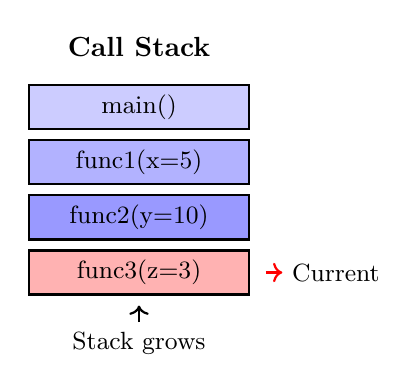
\begin{tikzpicture}[scale=0.7]
        \node at (2,5.5) {\textbf{Call Stack}};

        % Stack frames
        \draw[thick, fill=blue!20] (0,4) rectangle (4,4.8);
        \node at (2,4.4) {\small main()};

        \draw[thick, fill=blue!30] (0,3) rectangle (4,3.8);
        \node at (2,3.4) {\small func1(x=5)};

        \draw[thick, fill=blue!40] (0,2) rectangle (4,2.8);
        \node at (2,2.4) {\small func2(y=10)};

        \draw[thick, fill=red!30] (0,1) rectangle (4,1.8);
        \node at (2,1.4) {\small func3(z=3)};

        \draw[->, thick, red] (4.3,1.4) -- (4.6,1.4);
        \node[right] at (4.6,1.4) {\small Current};

        \draw[->, thick] (2,0.5) -- (2,0.8);
        \node[below] at (2,0.5) {\small Stack grows};
      \end{tikzpicture}
    \end{column}
  \end{columns}
\end{frame}

\begin{frame}{Heap Memory}
  \begin{columns}
    \begin{column}{0.5\textwidth}
      \begin{block}{Characteristics}
        \begin{itemize}
          \item Dynamic memory allocation
          \item Objects with longer lifetimes
          \item Larger capacity (GBs)
          \item Slower than stack
          \item Manual (C/C++) or GC (Java/Python)
        \end{itemize}
      \end{block}

      \vspace{0.3cm}

      \begin{block}{Memory Management}
        \textbf{C/C++:} Manual \\
        \texttt{malloc/free}, \texttt{new/delete}

        \vspace{0.2cm}

        \textbf{Java/Python:} Automatic \\
        Garbage collection
      \end{block}
    \end{column}
    \begin{column}{0.45\textwidth}
      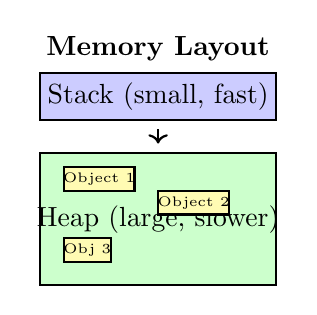
\begin{tikzpicture}[scale=0.6]
        \node at (2.5,6) {\textbf{Memory Layout}};

        % Stack section
        \draw[thick, fill=blue!20] (0,4.5) rectangle (5,5.5);
        \node at (2.5,5) {Stack (small, fast)};

        % Arrow
        \draw[->, thick] (2.5,4.3) -- (2.5,4);

        % Heap section
        \draw[thick, fill=green!20] (0,1) rectangle (5,3.8);
        \node at (2.5,2.4) {Heap (large, slower)};

        % Objects in heap
        \draw[thick, fill=yellow!30] (0.5,3) rectangle (2,3.5);
        \node at (1.25,3.25) {\tiny Object 1};

        \draw[thick, fill=yellow!30] (2.5,2.5) rectangle (4,3);
        \node at (3.25,2.75) {\tiny Object 2};

        \draw[thick, fill=yellow!30] (0.5,1.5) rectangle (1.5,2);
        \node at (1,1.75) {\tiny Obj 3};
      \end{tikzpicture}
    \end{column}
  \end{columns}

  \vspace{0.3cm}

  \begin{alertblock}{Common Issues}
    \textbf{C/C++:} Memory leaks, dangling pointers \\
    \textbf{Java/Python:} Shared references, unexpected mutations
  \end{alertblock}
\end{frame}

\begin{frame}[fragile]{Pointers and References}
  \begin{columns}
    \begin{column}{0.48\textwidth}
      \begin{exampleblock}{C++ Pointers}
        \begin{lstlisting}[language=C++,basicstyle=\tiny\ttfamily]
int x = 10;
int* ptr = &x;  // Pointer to x

*ptr = 20;      // Modify via pointer
cout << x;      // 20

// Heap allocation
int* arr = new int[100];
arr[0] = 5;
delete[] arr;   // Must free!

// Dangling pointer (BAD!)
int* p = new int(42);
delete p;
cout << *p;     // Undefined!
        \end{lstlisting}
      \end{exampleblock}
    \end{column}
    \begin{column}{0.48\textwidth}
      \begin{exampleblock}{Python References}
        \begin{lstlisting}[language=Python,basicstyle=\tiny\ttfamily]
# Objects are references
list1 = [1, 2, 3]
list2 = list1      # Same reference!

list2.append(4)
print(list1)       # [1, 2, 3, 4]

# To copy:
list3 = list1.copy()  # Shallow copy
list3.append(5)
print(list1)       # [1, 2, 3, 4]

# Deep copy for nested structures
import copy
nested = [[1, 2], [3, 4]]
deep = copy.deepcopy(nested)
        \end{lstlisting}
      \end{exampleblock}
    \end{column}
  \end{columns}

  \vspace{0.3cm}

  \begin{block}{Practice}
    \textbf{C/C++:} Allocate/free arrays, avoid leaks and dangling pointers \\
    \textbf{Java/Python:} Understand when objects are shared and mutated
  \end{block}
\end{frame}

%----------------------------------------------------------------------------------------
%    DEBUGGING AND TESTING
%----------------------------------------------------------------------------------------
\section{Debugging and Testing}

\begin{frame}{Debugging Strategies}
  \begin{columns}
    \begin{column}{0.48\textwidth}
      \begin{block}{Essential Tools}
        \begin{itemize}
          \item \textbf{Debugger}: Breakpoints, step through, watch variables
          \item \textbf{Assertions}: Capture invariants early
          \item \textbf{Logging}: Strategic print statements
          \item \textbf{Binary search}: Isolate bug location
        \end{itemize}
      \end{block}

      \vspace{0.3cm}

      \begin{alertblock}{Don't Just Print!}
        Use a proper debugger:
        \begin{itemize}
          \item Set breakpoints
          \item Inspect variable state
          \item Step line by line
          \item Understand execution flow
        \end{itemize}
      \end{alertblock}
    \end{column}
    \begin{column}{0.48\textwidth}
      \begin{block}{Debugging Process}
        \begin{enumerate}
          \item \textbf{Reproduce}: Minimal test case
          \item \textbf{Isolate}: Which function fails?
          \item \textbf{Inspect}: Variable values at failure
          \item \textbf{Hypothesize}: What could cause this?
          \item \textbf{Test}: Verify hypothesis
          \item \textbf{Fix}: Apply solution
          \item \textbf{Validate}: Ensure fix works
        \end{enumerate}
      \end{block}

      \vspace{0.2cm}

      \begin{exampleblock}{Tools by Language}
        \textbf{C/C++:} gdb, lldb, valgrind \\
        \textbf{Java:} JUnit, debugger \\
        \textbf{Python:} pdb, unittest, pytest
      \end{exampleblock}
    \end{column}
  \end{columns}
\end{frame}

\begin{frame}[fragile]{Testing Best Practices}
  \begin{columns}
    \begin{column}{0.48\textwidth}
      \begin{block}{Testing Principles}
        \begin{itemize}
          \item Start with unit tests
          \item Test edge cases
          \item Small and large inputs
          \item Property-based thinking
          \item Measure performance
        \end{itemize}
      \end{block}

      \vspace{0.2cm}

      \begin{exampleblock}{Edge Cases to Test}
        \begin{itemize}
          \item Empty input
          \item Single element
          \item Duplicates
          \item Negative numbers
          \item Boundary values
          \item Maximum size
        \end{itemize}
      \end{exampleblock}
    \end{column}
    \begin{column}{0.48\textwidth}
      \begin{exampleblock}{Python Unit Test}
        \begin{lstlisting}[language=Python,basicstyle=\tiny\ttfamily]
import unittest

class TestArrayOps(unittest.TestCase):
    def test_reverse_normal(self):
        arr = [1, 2, 3, 4]
        reverse(arr)
        self.assertEqual(arr, [4, 3, 2, 1])

    def test_reverse_empty(self):
        arr = []
        reverse(arr)
        self.assertEqual(arr, [])

    def test_reverse_single(self):
        arr = [1]
        reverse(arr)
        self.assertEqual(arr, [1])

    def test_reverse_property(self):
        arr = [1, 2, 3]
        reverse(reverse(arr))
        self.assertEqual(arr, [1, 2, 3])

if __name__ == '__main__':
    unittest.main()
        \end{lstlisting}
      \end{exampleblock}
    \end{column}
  \end{columns}
\end{frame}

%----------------------------------------------------------------------------------------
%    ONLINE JUDGES
%----------------------------------------------------------------------------------------
\section{Using Online Judges}

\begin{frame}{Online Judge Platforms}
  \begin{columns}
    \begin{column}{0.48\textwidth}
      \begin{block}{Popular Platforms}
        \begin{itemize}
          \item \textbf{LeetCode}: Interview prep
          \item \textbf{HackerRank}: Competitions, hiring
          \item \textbf{Codeforces}: Competitive programming
          \item \textbf{AtCoder}: Japanese CP platform
          \item \textbf{TopCoder}: Algorithms, marathons
        \end{itemize}
      \end{block}

      \vspace{0.3cm}

      \begin{block}{Benefits}
        \begin{itemize}
          \item Immediate feedback
          \item Test against edge cases
          \item Compare solutions
          \item Track progress
          \item Build problem-solving patterns
        \end{itemize}
      \end{block}
    \end{column}
    \begin{column}{0.48\textwidth}
      \begin{block}{Problem-Solving Approach}
        \begin{enumerate}
          \item \textbf{Read} carefully, note constraints
          \item \textbf{Design} algorithm with complexity
          \item \textbf{Implement} cleanly
          \item \textbf{Test} edge cases manually
          \item \textbf{Submit} and iterate
          \item \textbf{Reflect} on solution
          \item \textbf{Document} patterns learned
        \end{enumerate}
      \end{block}

      \vspace{0.2cm}

      \begin{alertblock}{Avoid Pitfalls}
        \begin{itemize}
          \item Don't just copy solutions
          \item Re-implement after understanding
          \item Pay attention to constraints
          \item Learn the pattern, not just the answer
        \end{itemize}
      \end{alertblock}
    \end{column}
  \end{columns}
\end{frame}

\begin{frame}{Common Problem Patterns}
  \begin{center}
    \begin{tabular}{l|p{4cm}|p{4cm}}
      \toprule
      \textbf{Pattern} & \textbf{Description} & \textbf{Example Problems} \\
      \midrule
      Two Pointers & Use two indices moving through data & Palindrome, pair sum \\
      \midrule
      Sliding Window & Fixed/variable size window & Max subarray sum \\
      \midrule
      Fast \& Slow Pointers & Detect cycles, find middle & Linked list cycle \\
      \midrule
      Stack & LIFO for matching/parsing & Valid parentheses \\
      \midrule
      BFS/DFS & Graph/tree traversal & Level-order, paths \\
      \midrule
      Binary Search & Divide search space & Search sorted array \\
      \bottomrule
    \end{tabular}
  \end{center}

  \vspace{0.5cm}

  \begin{block}{Measuring Progress}
    \begin{itemize}
      \item Track time per problem
      \item Monitor success rate
      \item Count revisits until first-try success
      \item Categorize by topic and difficulty
    \end{itemize}
  \end{block}
\end{frame}

%----------------------------------------------------------------------------------------
%    SUMMARY
%----------------------------------------------------------------------------------------
\section{Summary}

\begin{frame}{Key Takeaways}
  \begin{block}{Language and Tools}
    \begin{itemize}
      \item Choose one language and master it (Python/Java for learning, C++ for performance)
      \item Understand memory management for your language
      \item Learn debugging tools and use them effectively
    \end{itemize}
  \end{block}

  \begin{block}{Core Programming Skills}
    \begin{itemize}
      \item Master control flow, loops, and avoid off-by-one errors
      \item Understand recursion: base case, recursive case, stack frames
      \item Know array and string fundamentals, including complexity
    \end{itemize}
  \end{block}

  \begin{block}{Memory Model}
    \begin{itemize}
      \item Stack: fast, limited, automatic (function frames)
      \item Heap: larger, slower, manual or GC (dynamic objects)
      \item Understand pointers/references and their implications
    \end{itemize}
  \end{block}

  \begin{block}{Practice and Testing}
    \begin{itemize}
      \item Write tests for every function (edge cases!)
      \item Use online judges to build problem-solving patterns
      \item Implement data structures from scratch at least once
    \end{itemize}
  \end{block}
\end{frame}

\begin{frame}{Next Steps}
  \begin{block}{Moving Forward}
    With these foundations in place, you're ready to:
    \begin{itemize}
      \item Study linear data structures (arrays, linked lists, stacks, queues)
      \item Implement each structure from scratch
      \item Analyze time and space complexity
      \item Apply structures to real-world problems
      \item Build toward more complex structures (trees, graphs, hash tables)
    \end{itemize}
  \end{block}

  \vspace{0.5cm}

  \begin{exampleblock}{Recommended Practice}
    \begin{enumerate}
      \item Implement basic array operations (reverse, rotate, search)
      \item Write recursive solutions for factorial, Fibonacci, binary search
      \item Practice two-pointer and sliding window problems
      \item Solve 10-20 easy problems on LeetCode/HackerRank
      \item Build a simple stack/queue and test thoroughly
    \end{enumerate}
  \end{exampleblock}
\end{frame}

\begin{frame}[plain]
  \begin{center}
    {\Huge Thank You!}

    \vspace{1cm}

    {\large Questions?}

    \vspace{1cm}

    \textit{``The best way to learn data structures \\
    is to implement them yourself.''}
  \end{center}
\end{frame}

\end{document}
